\documentclass[]{article}

\usepackage[ngerman]{babel}
\usepackage{hyperref}
\usepackage{amsmath}
\usepackage{url}
\usepackage[numbers]{natbib}
\usepackage{graphicx}
\usepackage[nottoc]{tocbibind} % for adding Bibliography to table of contents
\usepackage{nameref}
\usepackage{siunitx}

%opening
\title{Oszilloskop mittels Mikrocontroller}
\author{Len-Marvin Adler, Deniz}

\begin{document}

\maketitle
\thispagestyle{empty}
\clearpage
\tableofcontents
\thispagestyle{empty}
\clearpage

\pagenumbering{roman}
\setcounter{page}{3}
\section*{Abkürzungen}
\addcontentsline{toc}{section}{\protect\numberline{}Abkürzungen}
% Abkürzungen
\begin{description}
	\item[ADC]
	Analog Digital Converter
	
	\item[GPIO]
	General Purpose Input Output

	\item[IDR]
	Input Data Register
	
	\item[Opamp]
	Operational Amplifier - Operationsverstärker

	\item[LCD]
	Liquid Crystal Display

	\item[TFT]
	Thin Film Transistor
\end{description}
\clearpage

\pagenumbering{arabic}
\setcounter{page}{1}
%% content of sections is written in the included files
%% 1.
\section{Einleitung}

Ein Oszilloskop ist ein Messgerät, dass in seiner Grundfunktion Spannungen
über einen Zeitverlauf lang messen und darstellen kann. \newline
Diese Darstellung erfolgt auf einem Display \cite{KnowUrOscilloscope}. \newline
%\begin{figure}[htpb]
%	\centering
%	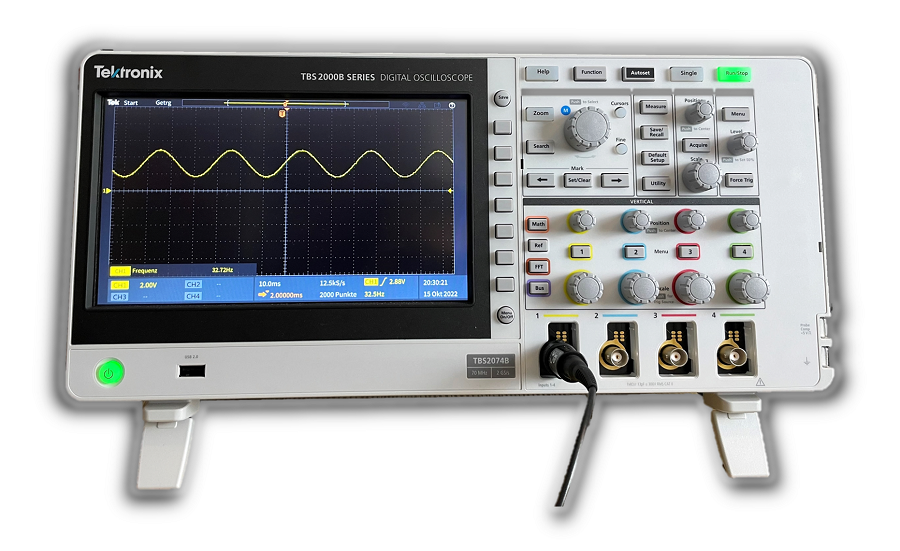
\includegraphics[width=\textwidth,height=6cm,keepaspectratio=true]{images/OszilloskopBeispiel.png}
%	\caption{
%		Oszilloskop aus \cite{OscilloscopeBild}
%	}
%	\label{Label}
%\end{figure} \newline
Komplexere Oszilloskope können häufig auch Messwerte persistent speichern oder die Skalierung der Achsen
ändern. Wegen letzterem lässt sich ein großer Umfang von Spannungswerten messen.
Durch diese Funktionen ist das Oszilloskop ein oft- und vielseitig verwendetes Messgerät
in der Elektrotechnik \cite{ETechnikEinfach}. \newline \newline
In dieser Seminararbeit wollen wir unser eigenes Oszilloskop bauen, das die Grundfunktionen,
eine Zeit lang Spannungen  zu messen und darzustellen, erfüllen soll.
Hierfür werden zuerst die groben Komponenten und deren Zusammenspiel im selbstgebauten Oszilloskop erläutert.\newline
Danach wird auf die einzelnen Bauteile und ihre Funktion eingegangen und
zuletzt eine Messung eines einfachen Schwingkreises durchgeführt, um an diesen Messwerten zu begründen,
ob das Oszilloskop die Anforderungen erfüllt.  



%% 2.
\section{Vorraussetzungen}
\label{Vorraussetzungen}

%% What you need for building our oscilloscope
%% also reasoning for the devices

\subsection{Geräte}




\subsection{Zusammenspiel}

Alle Geräte zusammen sehen als Schaltplan so aus:
\begin{figure}[h]
	\centering
	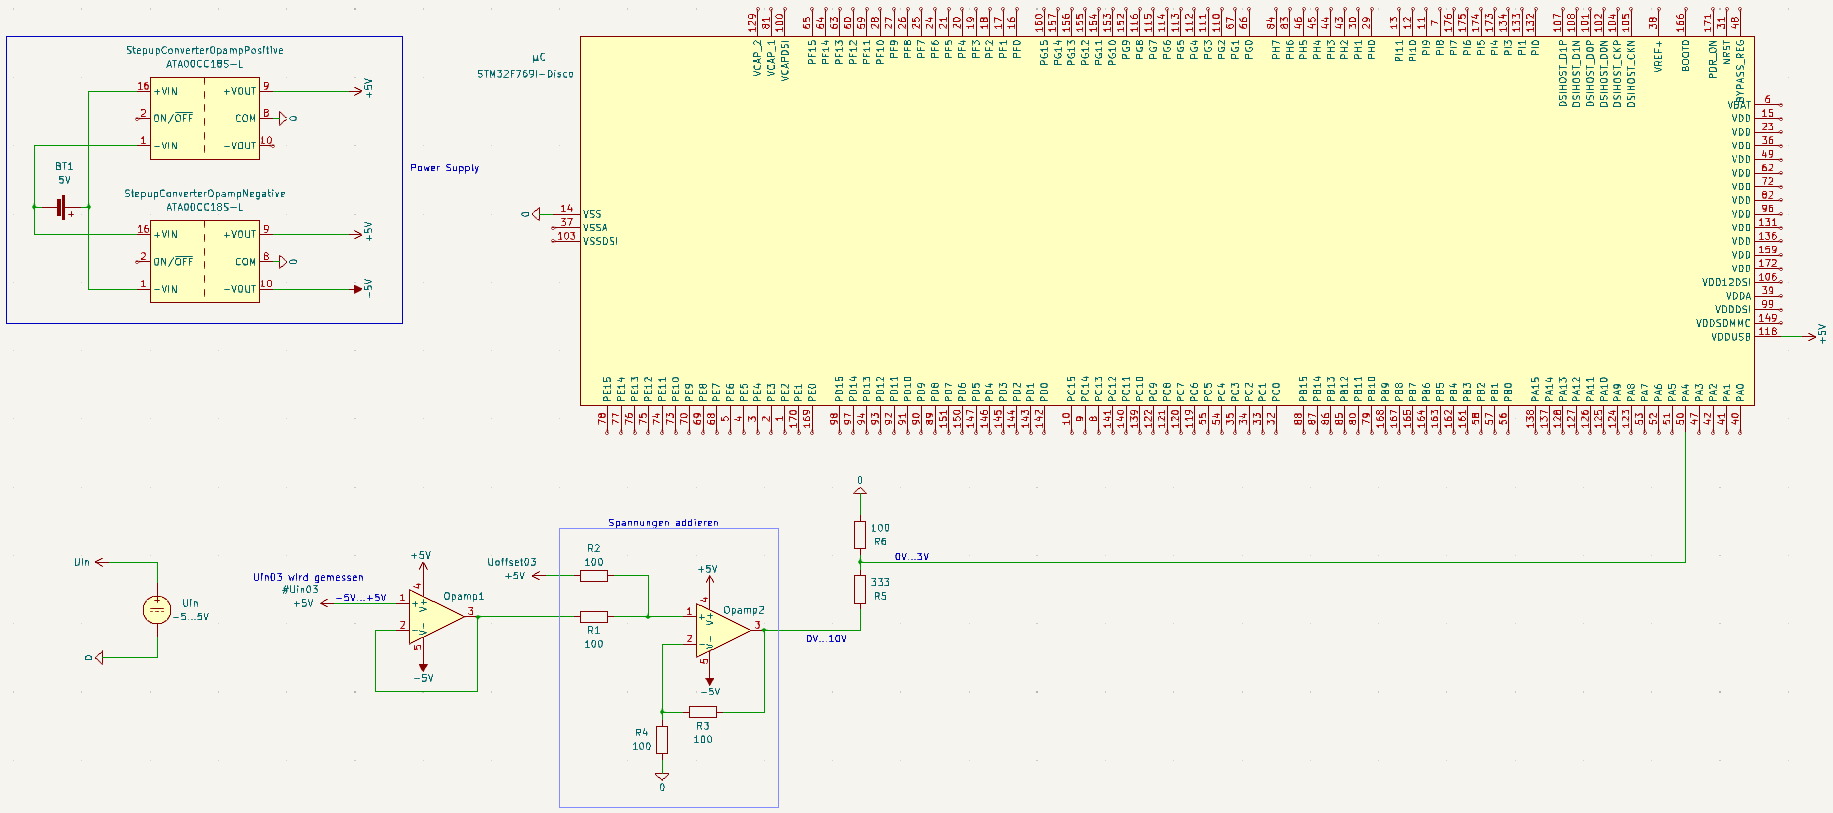
\includegraphics[width=\textwidth, scale=0.5]{images/schematic_opamps2.png}
	\caption{Schematischer Aufbau des Oszilloskops}
\end{figure}


Oszilloskop Eingang ist $U_{in}$ und der Ground $0$. \newline
Für die Messung, muss das Oszilloskop zur gemessenen Spannung parallel geschalten werden,
damit die Spannung am Oszilloskop die gleiche ist, wie die am gemessenen Stromkreis.

\subsubsection{Idee}
Die Eingangsspannung $U_{in}$ liegt im Intervall $[-15, 15] V$,
der GPIO Pin des Mikrocontrollers erlaubt allerdings nur $[0, 3.3] V$. \newline
Folglich muss die Eingangsspannung dahingehend bereinigt werden.
\newline \newline
Hierfür bringen wir die Eingangsspannung erstmal in den positiven Bereich, indem wir
eine Offset Spannung $U_{offset} = 15V$, mithilfe eines Nicht-invertierten Summerverstärkers, erläutert in \ref{Addition einer Offset-Spannung}, dazu addieren. \newline
Der Spannungsbereich ändert sich dadurch zu $[0, 30] V$.
Dieser muss nun lediglich, mithilfe eines Spannungsteilers, siehe \ref{Spannungsteiler}, zu $[0, 3.3] V$ aufgeteilt werden.
Damit der gemessene Stromkreis durch das Oszilloskop nicht belastet wird, muss noch ein Bauteil mit einer hohen Eingangsimpedanz, erläutert in \ref{Unbelastete Eingangsspannung}, vor das ganze Netzwerk geschalten werden.


\subsubsection{Stromversorgung}
Der Mikrocontroller wird über USB mit $5V$ versorgt.
Die beiden Opamps werden durch eine Batterie mithilfe von Stepup Convertern versorgt.

Später werden die einzelnen Schritte ausführlicher erläutert und begründet.





%% 3.
\section{Eingangsspannung bereinigen}
\label{Eingangsspannung bereinigen}

%% Describes our Opamps and Voltage divider
%% also reasoning for choosing those specific
%% values of resistor, power supply, etc.
Der GPIO Pin aus \ref{Mikrocontroller}, an dem die Spannung mithilfe eines Mikrocontrollers gemessen wird,
kann nur Spannung im Bereich $[0, 3.3]V$ messen.
Das Oszilloskop soll allerdings einen größeren Spannungsbereich $[-5, 5]V$ messen können.
Daher wird nun die Eingangsspannung bereinigt, sodass sie den Anforderungen des GPIO Pin genügt.

\subsection{Unbelastete Eingangsspannung}
\label{Unbelastete Eingangsspannung}
Der Stromkreis, der gemessen wird, soll nicht belastet werden, daher wird ein Opamp mit
hoher Eingangsimpedanz und einem Verstärkungsfaktor von $1$ benutzt.
Dies wird durch eine Rückkopplung des Ausgangs an den invertierten Eingang des Opamps erreicht.
\begin{figure}[h]
	\centering
	\includegraphics[width=0.7\textwidth]{images/schematic\_teil1\_unbelastet\_opamp.png}
	\caption{Schaltplan um den Eingangsstrom nicht zu belasten, Ausschnitt aus \ref{Gesamte_Schematic}}
\end{figure}


\subsection{Addition einer Offset-Spannung}
\label{Addition einer Offset-Spannung}

Nun gilt es den Spannungsbereich von $[-5, 5]V$ auf $[0, 10]V$ zu legen.
Dafür wird eine Offset-Spannung $U_{offset}$, die aus einem $V_{CC}$ Pin
des Mikrocontrollers stammt und mithilfe des Stepup Spannungsreglers auf $5V$ gebracht wird, zur Eingangsspannung dazu addiert.
Dies geschieht mit einem Nichtinvertierenden Summierverstärker, also ein Opamp der extern mit
Spannungsteilern, gemäß \autoref{fig:Opamp_Adder}, beschalten ist.
Der Opamp arbeitet also mit Spannungen im Bereich $[-5,10]V$,
daher muss der Bereich der Versorgungsspannung mindestens diese Spannungswerte enthalten.
Experimentell hat sich herausgestellt, dass der \textit{TS912IN} funktioniert, solange die Eingangsspannung
unterhalb von $1.7V$ der Versorgungsspannung liegt.
Daher wird für den Opamp großzügig eine positive Versorgungsspannung von $V^+_{CC} = 15V$ und eine 
negative von $V^-_{CC} = -15V$ gewählt.
Für die maximale Eingangsspannung gilt $\max(U_{in}) + U_{offset} = 5V + 5V = 10V < (15V - 1.7V)$
und für die minimale gilt $\min(U_{in}) + U_{offset} = -5V + 5V = 0V$.
Der Opamp funktioniert also für die definierte Eingangs- und Offsetspannung. \newline
Es gilt, laut \cite{Opamp_adder}, für die Ausgangsspannung $U_3$ des Opamps:
\begin{align*}
U_3 &= (U_{in} \cdot \frac{R_2}{R_1 + R_2} + U_{offset} \cdot \frac{R_1}{R_1 + R_2}) \cdot(1 + \frac{R_4}{R_3}) \\
	&= (U_{in} \cdot \frac{1}{2} + U_{offset} \cdot \frac{1}{2}) \cdot 2 \\
	&= U_{in} + U_{offset}
\end{align*}

\begin{figure}[h!]
	\centering
	\includegraphics[width=0.7\textwidth]{images/schematic\_teil2\_adder.png}
	\caption{Addition von $U_{in}$ und $U_{offset}$, Ausschnitt aus \ref{Gesamte_Schematic}}
	\label{fig:Opamp_Adder}
\end{figure}

%Eine Messung der Spannung von $U_{in}$ und $U_3$ mittels eines kommerziellen Oszilloskops zeigt,
%für eine Wechselspannung mit Amplitude $5V$, erfolgreich $U_3 = U_{in} + U_{offset}$:
%\begin{figure}[h!]
%	\centering
%	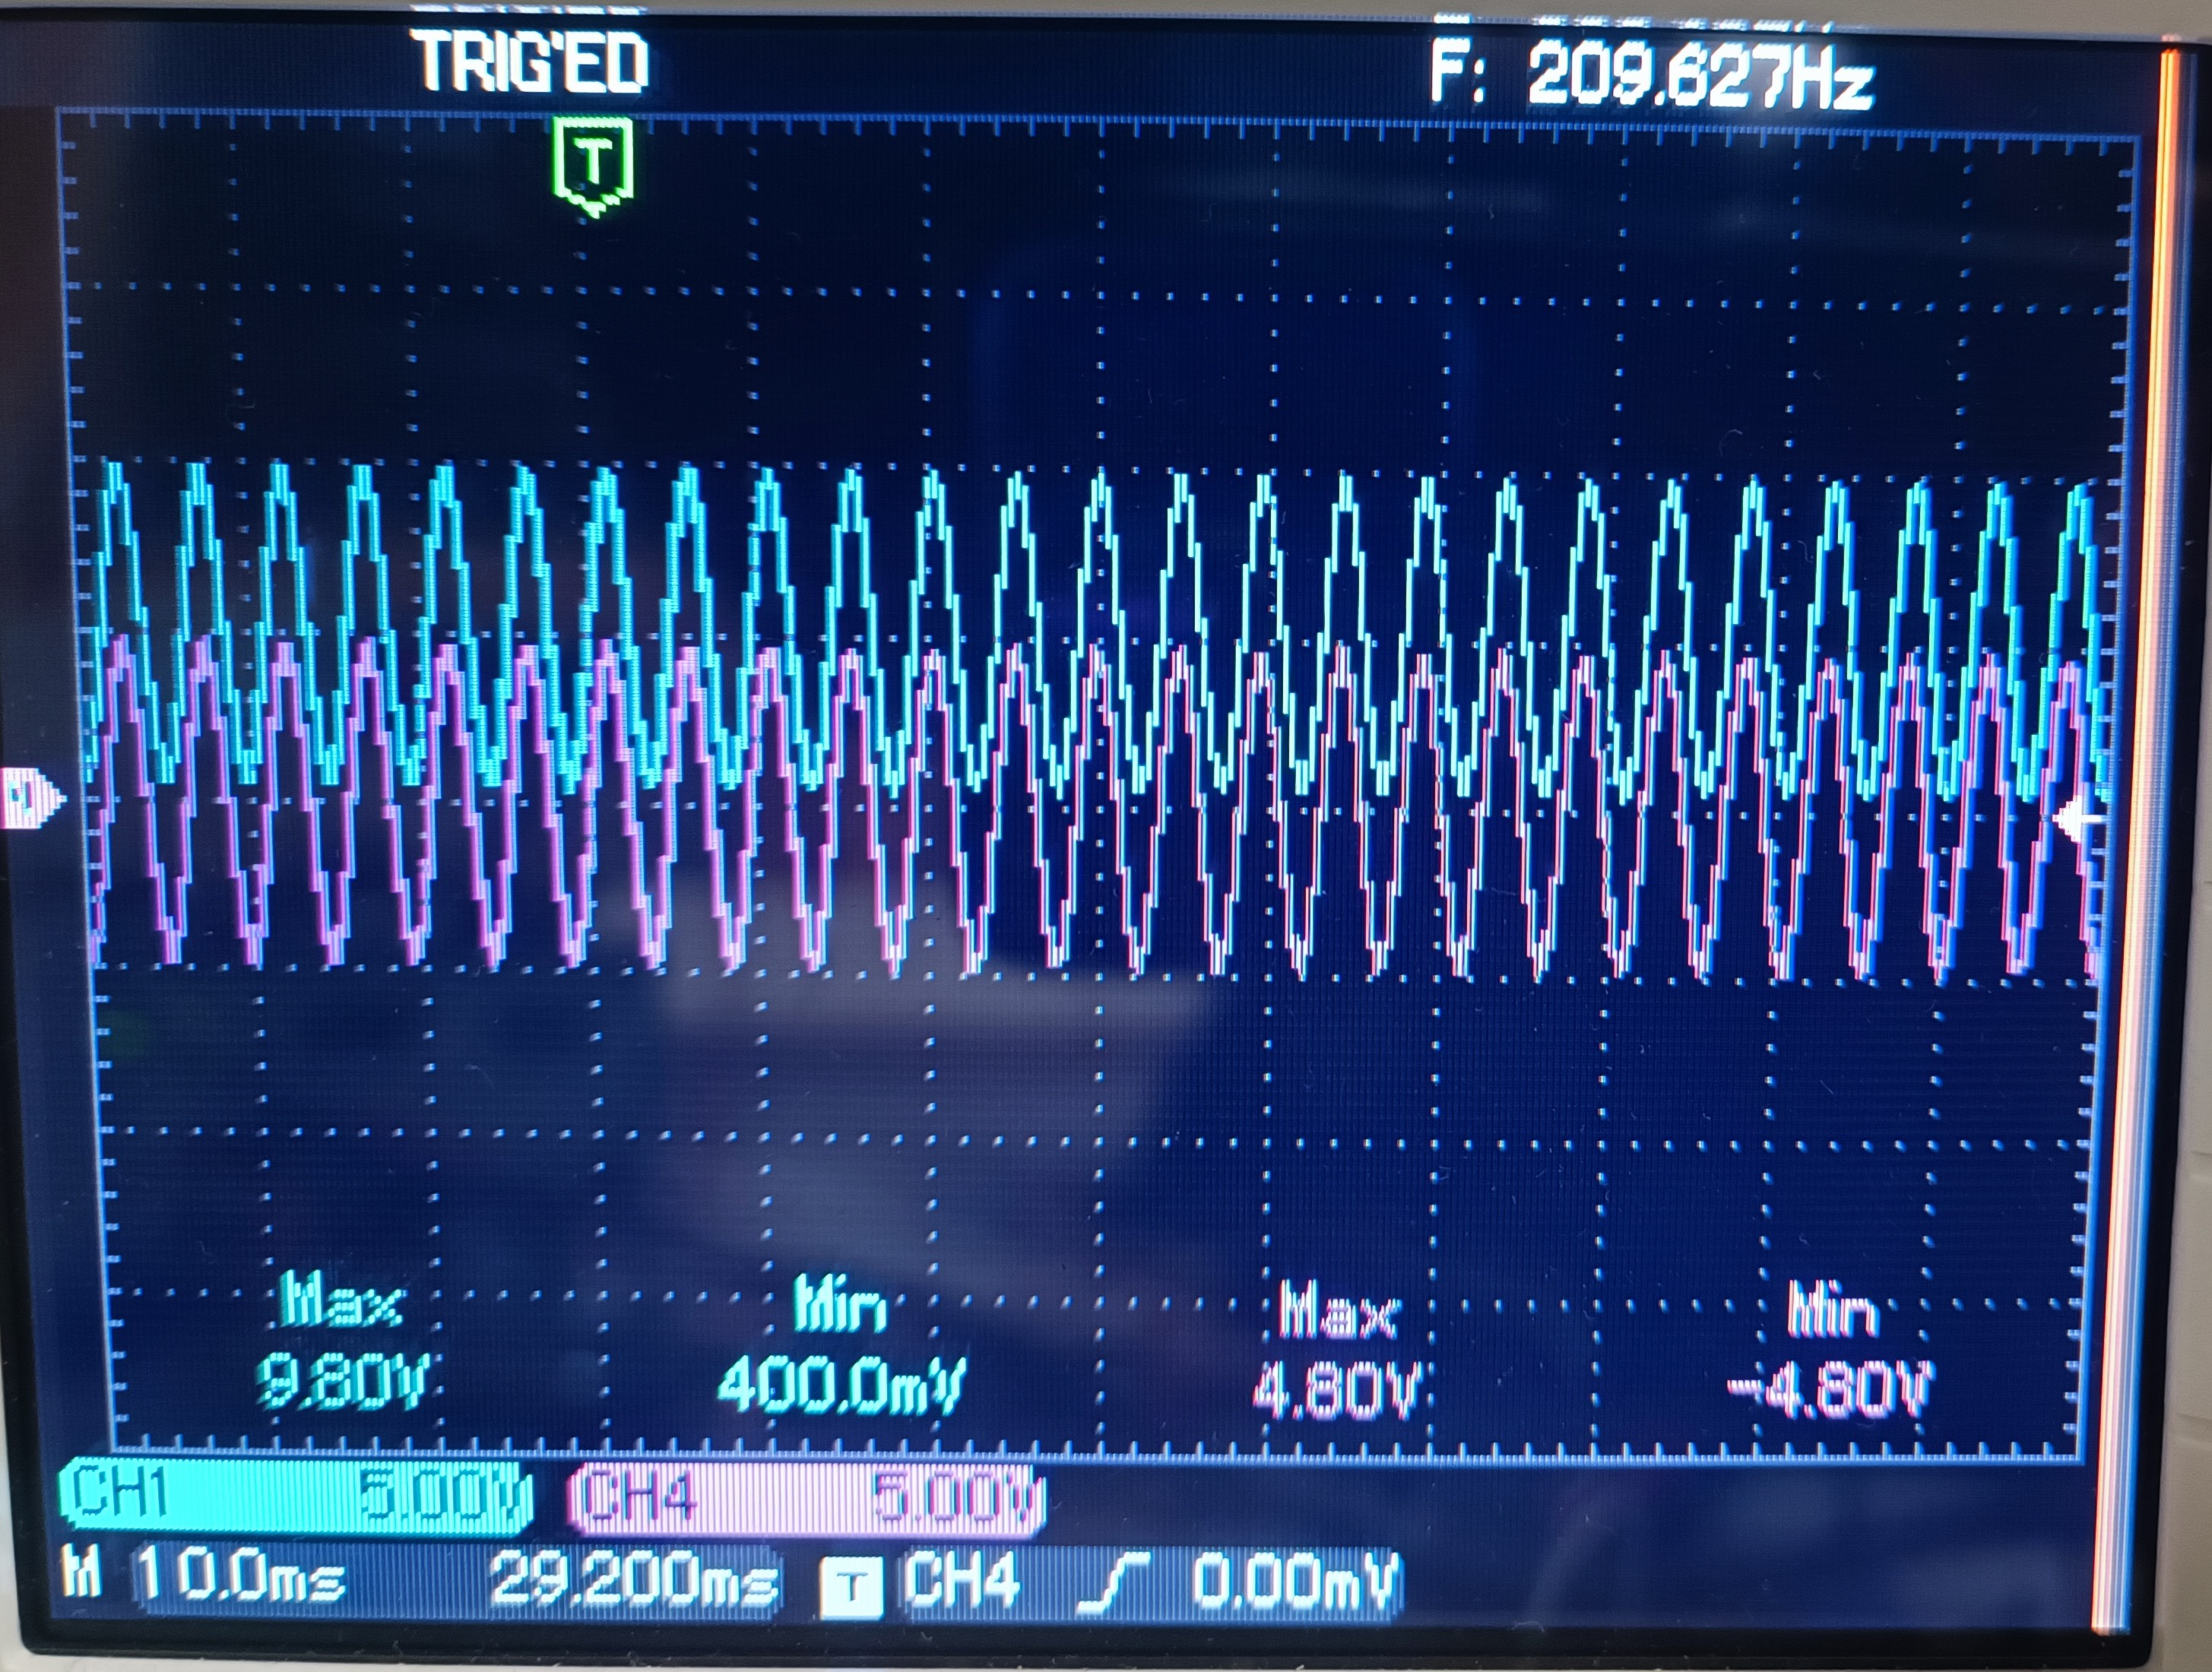
\includegraphics[width=0.7\textwidth]{images/messung_adder.jpg}
%	\caption{Messung von $U_{in}$ (lila) und $U_3$ (blau)}
%\end{figure}

\subsection{Spannungsteiler}
\label{Spannungsteiler}

Zuletzt wird die Spannung $U_3$, welche aus \textit{Opamp2} gegeben wird, geteilt, sodass
sie im Bereich $[0, 3.3]V$ für den GPIO Pin liegt.
Der Spannungsteiler $(R_5, R_6)$ teilt $U_3$ dabei zu
$U_{GPIO} = U_3 \cdot \frac{R_6}{(R_5 + R_7) + R_6} = U_3 \cdot \frac{100 \Omega}{330 \Omega}$. \newline
Dadurch ergibt sich ein Spannungsbereich für $U_{GPIO}$ von
$[0, 10 \cdot \frac{100}{330}]V = [0, 3.3]V$.
\begin{figure}[h!]
	\centering
	\includegraphics[scale=0.7]{images/schematic\_teil3\_spannungsteiler.png}
	\caption{Spannungsteiler zu $U_{GPIO}$, Ausschnitt aus \ref{Gesamte_Schematic}}
\end{figure}
\newline
Die bereinigte Spannung $U_{GPIO}$ wird nun an den GPIO Pin des Mikrocontrollers angeschlossen.





%% 4.
\section{Mikrocontroller}
\label{Mikrocontroller}

%% Describes STM32F769I-DISCO, GPIO, registers, etc.
%% also some internal processing values
%% e.g. Taktrate am GPIO,
%%      Genauigkeit beim messen am GPIO
Die Spannungswerte lassen sich allerdings noch nicht messen oder darstellen.
Daher wird ein Bauteil benötigt, das die Spannungswerte digital darstellen kann.
Hierfür wird ein Mikrocontroller verwendet, der durch seine GPIO Pins und eingebauten ADC die Werte digital speichern kann.
Der STM32F769I-DISCO eignet sich, weil dieser zusätzlich ein integriertes 4 Zoll LCD Display
besitzt\cite{MikroControllerDatasheet_1}.
Durch die Bibliothek \textit{EmbSysLib} \cite{EmbSysLib}, wird die Software Implementierung des Displays zusätzlich
erleichtert. Zusätzlich wird das STM32F769-Disco Extension Board verwendet, um mehr
Anschlussmöglichkeiten am Mikrocontroller zu haben \cite{MikrocontrollerExtension}.
Im Folgenden werden die verwendeten Komponenten des Mikrocontrollers erläutert.

\subsection{GPIO}
Der STM32F769I-DISCO besitzt pro GPIO Pin vier 32-Bit Konfigurationsregister, zwei 32-Bit Datenregister
und ein 32-Bit Set-/Reset-Register \cite{MikroControllerDatasheet_1}.
Diese werden gebraucht um Daten zu lesen und zu senden.
\textit{General Purpose} bedeutet, dass die Pins für unterschiedlichste Zwecke für
Input/Output programmiert werden können \cite{RPI-GPIO}. \newline
Das Oszilloskop ist ein Messgerät, daher wird nur die Input Funktionalität des GPIO benötigt.
Um die analogen Spannungen messen und ausgeben zu können, müssen sie als digitaler Wert
im Mikrocontroller vorliegen. \newline
Die Umwandlung von analogem zu digitalem Wert übernimmt der ADC\cite{MikroControllerDatasheet_1}.
Deshalb muss unser Messeingang an einem GPIO Pin mit ADC Anschluss liegen, der \textit{ADC1} an GPIO Pin
\textit{PA4} eignet sich hierfür\cite{STM32F769_PinLayout, MikroControllerDatasheet_Pins}.
Am Extension Board liegt dieser Pin an Sensor Port \textit{S2-2} \cite{MikrocontrollerExtension}.


\subsection{ADC}

Der Mikrocontroller verwendet einen 12-Bit Analog-Digital-Converter (ADC).
Die analogen Werte werden also mit einer Auflösung von 12-Bit am \textit{PA4} gelesen und dann
in das 16-Bit Input-Data-Register (IDR) des Pins als digitaler Wert
geschrieben\cite{MikroControllerDatasheet_1}.
Deshalb kann der ADC zwischen $2^{12} = 4096$ verschiedene Spannungswerte im erlaubten Spannungsbereich,
$0V$ bis $3.3V$, am Pin messen\cite{MikroControllerDatasheet_1}.
Das Oszilloskop verwendet am Pin allerdings nur bis $3V$, dadurch ist das Teilungsverhältnis des Spannungsteilers
aus \ref{Spannungsteiler} einfacher zu berechnen. \newline
Hierbei sei gesagt, dass die Werte im IDR nicht direkt mit den gemessenen Spannungen korrellieren,
da der ADC einen Hex Wert zuweist, der im Bereich $0$ bis $4095$ liegt, dieser Wert aber nichts mit
dem Spannungswert zu tun hat. \newline
Ferner lässt sich die Grenze der Genauigkeit am ADC ausrechnen, also welcher Spannungsbereich denselben
Wert im IDR zugewiesen bekommt. \newline
Sei $\Delta U$ die Differenz zwischen zwei Spannungen, deren Hex-Werte im IDR sich um $1$
unterscheiden und $Hex = 4096$ die Anzahl der verschiedenen Werte im IDR,
dann
$$\Delta U = \frac{3.3V}{Hex} = 0.8mV$$
Das bedeutet, alle $0.8mV$ am Pin, verändert sich der IDR Wert. \newline
Folglich kann das Oszilloskop nicht genauer als auf $0.8mV$ messen.
\newline \newline
In \textit{EmbSysLib/Example/Src/Board/STM32F769-Discovery/config.h} wird nun ein
\texttt{Timer\_Mcu timer(Timer\_Mcu::TIM\_11, 100L)} Objekt erstellt\cite{EmbSysLib}. \newline
\texttt{100L} gibt an, dass alle $100\mu s$ ein Timer Interrupt ausgeführt werden soll.
Ein Timer Interrupt ruft dann die \texttt{virtual void TaskManager::Task::update()} Methode auf,
welche in einer abgeleiteten Klasse \texttt{MyTimer} überschrieben wurde EIGENEN CODE ZITIEREN.
Diese Methode liest einen Wert aus IDR und schreibt diesen in ein Array
für die spätere Darstellung. \newline
Ein Wert wird alle $100\mu s$ gemessen, also
$$
\frac{1 \text{Wert}}{100 \mu s} \iff 10\frac{\text{Werte}}{ms}
\iff 10000 \frac{\text{Werte}}{s}
$$
Daraus folgt für die Frequenz $f$ der Messung
$$
f = 10000 \frac{1}{s} = 10 \si{\kilo\hertz}
$$

\subsection{Eingangsspannung berechnen}
Die Spannung am GPIO Pin \text{PA4} wird im Folgenden $U_{GPIO}$ genannt. \newline
Die Eingangsspannung wird als $U_{in}$ bezeichnet und die Spannung zwischen Opamp$_2$
und Spannungsteiler $(R_5, R_6)$ als $U_{vorST}$ angegeben.
\newline \newline
Die gemessene Spannung lässt sich wie folgt ausrechnen: \newline
Sei $U_{GPIO}$ die gemessene Spannung an \textit{PA4}, $Hex \in [0, 4095]$ der zugewiesene Wert im IDR
und $3V$ die maximale Spannung, die das Netzwerk aus \nameref{Schematic_all} an den \textit{PA4} gibt,
dann gilt
$$
	U_{GPIO} = \frac{Hex \cdot 3V}{4095}
$$
ist die Spannung an \textit{PA4} in Volt.
\newline \newline
Die Spannung $U_{GPIO}$ ist allerdings nicht die Eingangsspannung am Oszilloskop, die tatsächlich gemessen werden soll, da
das Opamp-Netzwerk aus \ref{Eingangsspannung bereinigen} diese, für den GPIO Pin, bereinigt.
Es gilt nun, diese Bereinigung Schritt für Schritt in der Software wieder zurückzurechnen, um die Eingangsspannung zu erhalten. \newline
Der Spannungsteiler aus \ref{Spannungsteiler} teilt $U_{vorST}$
zu $U_{GPIO}$, also gilt laut Spannungsteilerregel
$$
	U_{GPIO} = \frac{U_{vorST} \cdot 100 \Omega}{333 \Omega + 100 \Omega}
$$
Daraus folgt
$$
	U_{vorST} = \frac{U_{GPIO} \cdot (333 \Omega + 100 \Omega)}{100 \Omega}
$$
\newline\newline
Um dann die Eingangsspannung zu erhalten, muss man lediglich die Offset Spannung $U_{offset}$
von $U_{vorST}$ subtrahieren, es folgt
$$
	U_{in} = U_{vorST} - U_{offset}
$$
wobei $U_{in}$ die Eingangsspannung, die gemessen werden soll, darstellt.


\subsection{Display}

Das Display ist ein $4$-Zoll LCD-TFT-Display mit einer Auflösung von \newline $800 \times 472 \si{px}$
und einer Bildwiederholrate von 30\si{\hertz} \cite{MikroControllerDatasheet_1}.
Da für die Frequenz der Messung $10 \si{\kilo\hertz} > 30 \si{\hertz}$ gilt,
misst der Mikrocontroller deutlich schneller, als er die Messwerte darstellen könnte.
Die gemessenen Werte müssen dementsprechend zumindest temporär, bis zur Darstellung auf dem Display,
in einer Datenstruktur, z.B. einem Array, zwischengespeichert werden SIEHE EIGENEN CODE EINFÜGEN MIT FLAGS.
Sobald das Array gefüllt wurde, wird es ausgegeben. In der Zeit vom gefüllten Array bis zur
vollständigen Ausgabe ZEIT MESSEN UND HIERREIN SCHREIBEN wird das Array weder geleert noch überschrieben,
da sonst die alten Daten, die eventuell noch nicht ausgegeben wurden, verloren gehen.
Daher wird beim Oszilloskop der Fokus auf korrekt gemessene, aufeinanderfolgende Werte in einer
Stichprobe anstatt auf eine kontinuierliche Messung gelegt.



%% 5.
\section{Beispiel-Nutzung}

%% describes an exampe of Usage
%% schaltkreis, messwerte, etc.
%% von Schwingkreis (LC-Circuit)
Example

\subsection{Schwingkreis}


%% 6.
\section{Benchmarking}

\subsection{Messaufbau}
Wie wird unser Oszilloskop gebenchmarked

\subsection{Messdurchführung}

Wie wird die Messung mit Oszilloskop durchgeführt

\subsection{Messwerte}

Was für quantitative Werte gemessen wurden

\subsection{Auswertung}

Was das für unser Oszilloskop bedeutet



%% Benchmarking our oscilloscope
%% vs. a real/professional one
%% Taktrate, Genauigkeit, etc.


%% 7.
\section{Diskussion}

%% issues we faced or
%% issues oscilloscope has (maybe already in 6-Benchmarking)
Issues


%% 8.
\section{Fazit}

%% Schlusswort / final words
Das Oszilloskop misst akzeptabel gut im Bereich der Anforderungen, daher
kann es für Messungen in diesem Bereich eingesetzt werden.
Jedoch steht es einem kommerziellen Oszilloskopen im Triggering, Darstellungsbereich der Messung und 
in der Messfrequenz nach.
Es wird daher angeraten, es nicht für professionelle Messungen zu verwenden.
Für Hobbyprojekte, beziehungsweise um eine simple Spannungskurve zu sehen,
sollte das Oszilloskop dennoch ausreichen und man muss kein kommerzielles Gerät kaufen.

% Anhang, alles was zu groß ist kommt hier rein
%\addcontentsline{toc}{section}{\nameref{Anhang}}
\section*{Anhang}
\label{Anhang}

% list of all attachments
\begin{enumerate}[label=\textbf{A.\arabic*}]
	\item
		\label{Gesamte_Schematic}
		\begin{minipage}[]{\linewidth}
			\centering
			\includegraphics[width=\textwidth, scale=0.1]{images/schematic\_oszilloskop\_horizontal.png}
			\captionof{figure}{Schematischer Aufbau des Oszilloskops}
		\end{minipage}

	\item
		\label{Display_Code}
		Code für die Verwendung des Mikrocontrollers \newline
		\url{https://github.com/gooosz/Oscilloscope_Display.git}
\end{enumerate}



%% Bibliography
\bibliographystyle{plainnat}
\bibliography{bib/bibliography.bib}


\end{document}
